\documentclass[10pt,a4paper]{report}
\usepackage[utf8]{inputenc}
\usepackage[russian]{babel}
\usepackage[OT1]{fontenc}
\usepackage{amsmath}
\usepackage{amsfonts}
\usepackage{amssymb}
\usepackage{graphicx}
\author{Киселев Антон и Кенть Никита}
\title{Отчет по лабораторной работе по дисциплине: "Сети и системы передачи данных"\newline
тема: "Визуализация сигналов во временной и частотной области"}
\date{13.03.14}
\begin{document}
\maketitle
\pagebreak
\chapter{Теоретическая часть}
\section{Цель работы}
Познакомиться со средствами генерации сигналов и визуализации их спектров.
\section{Постановка задачи}
В командном окне MATLAB и в среде Simulink промоделировать чистый синусоидальный сигнал, 
так же синусоидальный сигнал с шумом. Получить их спектры.

\chapter{Ход работы}
\section{Алгоритм работы. Построение сигналов}
\begin{itemize}
\item Построение синусоидального сигнала без шумов
\item Вывод временной характеристики сигнала
\item Реализация  преобразования Фурье 
\item Построение графика спектральной плотности 
\item Построение зашумленного синусоидального сигнала  
\item Вывод временной характеристики полученного сигнала
\item Преобразования Фурье 
\item Построение графика спектральной плотности для зашумленного сигнала
\end{itemize}
\section{Код MATLAB}
function main()\newline
x=0:0.01:4*pi;\newline
t0 = 5;\newline
\%исходный сигнал\newline
y = sin(2*pi*f0*x);\newline
figure(1)\newline
plot(x(1:200),y(1:200))\newline
grid\newline
\%спектр исходного сигнала\newline
figure(2)\newline
spectrum = fft(y,1024);\newline
normspectrum = spectrum.*conj(spectrum)/1024;\newline
f=100*(0:1023)/1024;\newline
plot(f, normspectrum(1:1024))\newline
axis([0 max(f) 0 10])\newline
grid\newline
\%зашумленный сигнал\newline
ynoize = y+ 0.5*rand(size(x));\newline
figure(3)\newline
plot(x(1:200),ynoize(1:200));\newline
grid\newline
\%спектр зашумленного сигнала\newline
spectrum = fft(ynoize,1024);\newline
noizespectrum = spectrum.*conj(spectrum)/1024;\newline
figure(4)\newline
plot(f, noizespectrum())\newline
axis([0 max(f) 0 10])\newline
grid\newline
\section{Результаты работы}
В результате выполнения программы получились графики временной и частотной характеристик исходного и зашумленного синусоидальных сигналов. \newpage
\begin{figure}
\begin{center}
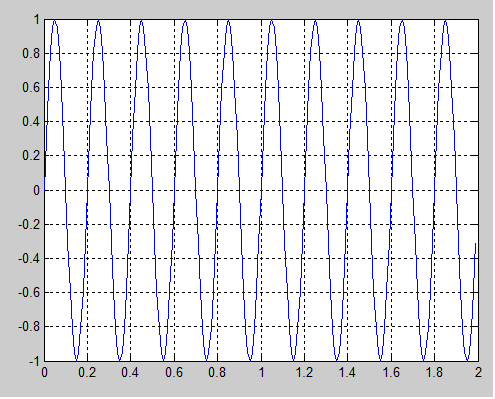
\includegraphics[angle=0, scale = 0.9]{1.png}\newline
рис. 1 Исходный сигнал\newline
\end{center}
\begin{center}
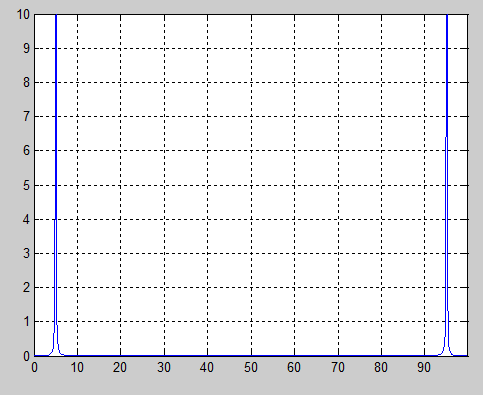
\includegraphics[angle=0, scale = 0.9]{2.png}\newline
рис. 2. Спектр исходного сигнала\newline
\end{center}
\end{figure}
\begin{figure}
\begin{center}
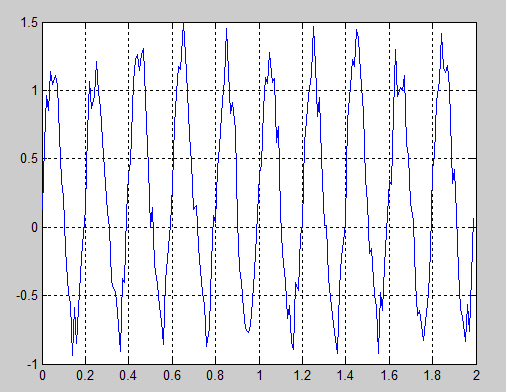
\includegraphics[angle=0, scale = 0.9]{3.png}\newline
рис. 3. Зашумленный сигнал\newline
\end{center}
\begin{center}
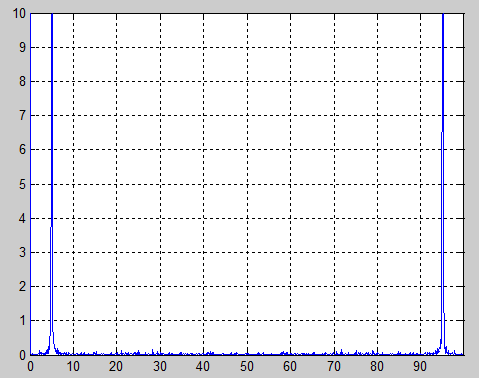
\includegraphics[angle=0, scale = 0.9]{4.png}\newline
рис. 4. Спектр зашумленного сигнала\newline
\end{center}
\end{figure}

\chapter{Построение спектров}
\section{Алгоритм работы}
\begin{itemize}
\item Построение полигармонического сигнала
\item Построение прямоугольного импульсного сигнала
\item Построение треугольного импульсного сигнала
\item Получение спектров этих сигналов
\item Создание моделей в Simulink
\end{itemize}
\section{Код MATLAB}
function laba5()\newline
x = 0:0.01:4*pi;\newline
f0 = 5;\newline
y = 0;\newline
for i=1:1:100\newline
    y=y+cos(i*x);\newline
end\newline
plot(x(1:100),y(1:100));\newline
figure(1)\newline
spectrum=fft(y,512);\newline
normspectrum=spectrum.*conj(spectrum)/512;\newline
f=100*(0:255)/512;\newline
figure(2)\newline
plot(f,normspectrum(1:256))\newline
axis([0 max(f) 0 10])\newline
grid \newline
figure(3)\newline
y1=square(x,50)\newline
plot(x(1:1000),y1(1:1000),'LineWidth',2);\newline
ylim([-1.2,1.2]);\newline
spectrum=fft(y1,512);\newline
normspectrum=spectrum.*conj(spectrum)/512;\newline
f1=100*(0:255)/512;\newline
figure(4)\newline
plot(f1,normspectrum(1:256))\newline
axis([0 max(f1) 0 10])\newline
grid \newline
y2=conv(y1,y1);\newline
figure(5)\newline
plot(x(1:1000),y2(1:1000),'LineWidth',2);\newline
grid\newline
spectrum=fft(y2,512);\newline
normspectrum=spectrum.*conj(spectrum)/512;\newline
f2=100*(0:255)/512;\newline
figure(6)\newline
plot(f2,normspectrum(1:256)/1000)\newline
axis([0 max(f2) 0 10])\newline
grid \newline
end\newline
\section{Результаты работы}
\begin{figure}
\begin{center}
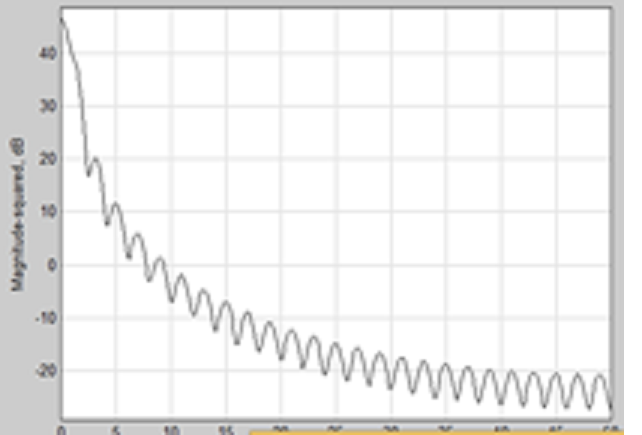
\includegraphics[angle=0, scale = 0.9]{5.png}\newline
рис. 5. спектр прямоугольного сигнала\newline
\end{center}
\end{figure}
\begin{figure}
\begin{center}
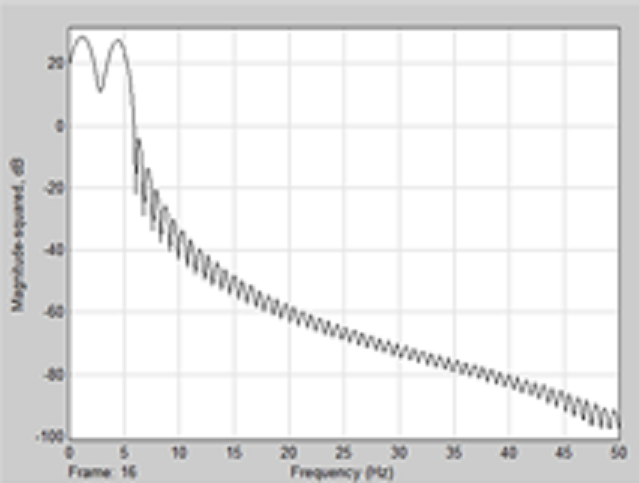
\includegraphics[angle=0, scale = 0.7]{6.png}\newline
рис. 6.спектр полигармонического сигнала\newline
\end{center}
\end{figure}
\begin{figure}
\begin{center}
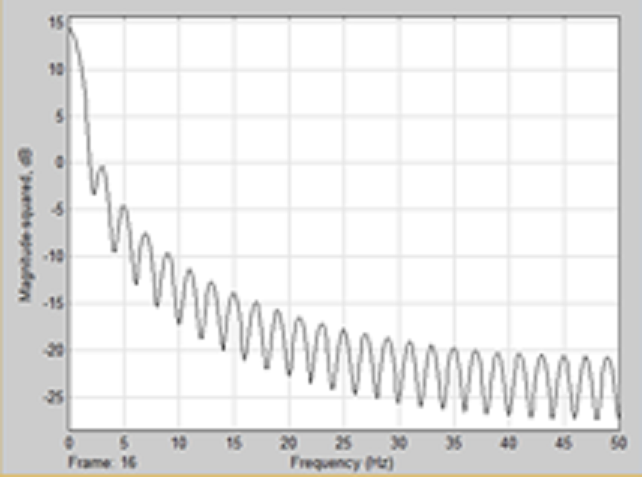
\includegraphics[angle=0, scale = 0.7]{7.png}\newline
рис. 7.спектр треугольного сигнала\newline
\end{center}
\end{figure}
\begin{figure}
\begin{center}
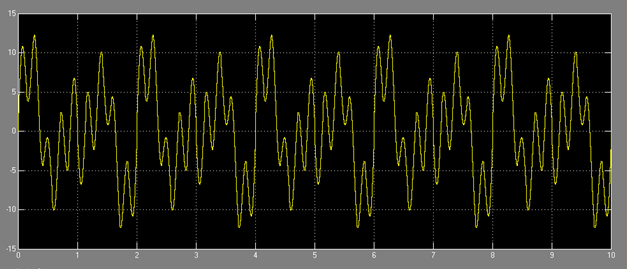
\includegraphics[angle=0, scale = 0.7]{8.png}\newline
рис. 8 полигармонический сигнал\newline
\end{center}
\end{figure}
\begin{figure}
\begin{center}
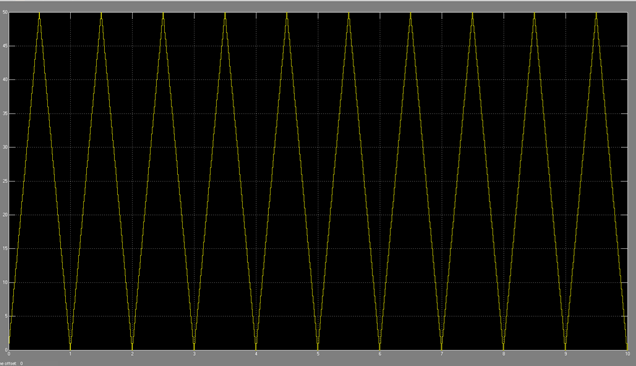
\includegraphics[angle=0, scale = 0.7]{9.png}\newline
рис. 9  треугольный сигнал\newline
\end{center}
\end{figure}
\begin{figure}
\begin{center}
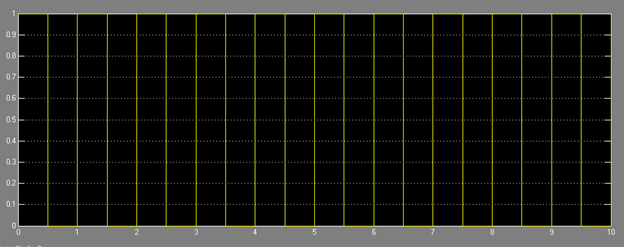
\includegraphics[angle=0, scale = 0.7]{10.png}\newline
рис. 10  прямоугольный сигнал\newline
\end{center}
\end{figure}


\begin{figure}
\begin{center}
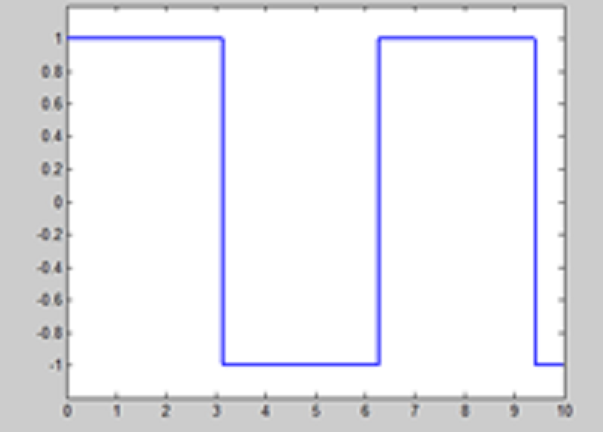
\includegraphics[angle=0, scale = 0.7]{11.png}\newline
рис. 11  прямоугольный сигнал\newline
\end{center}
\end{figure}

\begin{figure}
\begin{center}
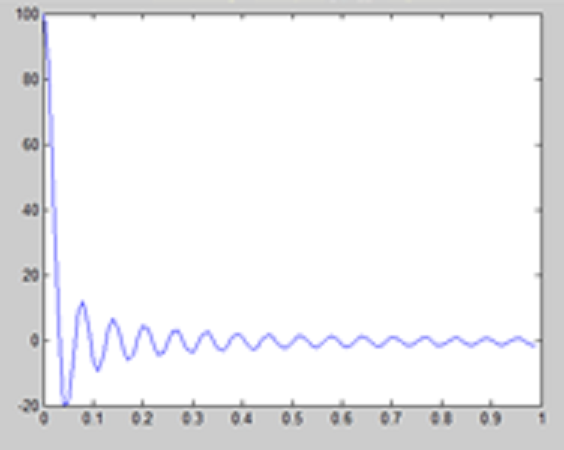
\includegraphics[angle=0, scale = 0.9]{12.png}\newline
рис. 12  полигармонический сигнал\newline
\end{center}
\end{figure}
\begin{figure}
\begin{center}
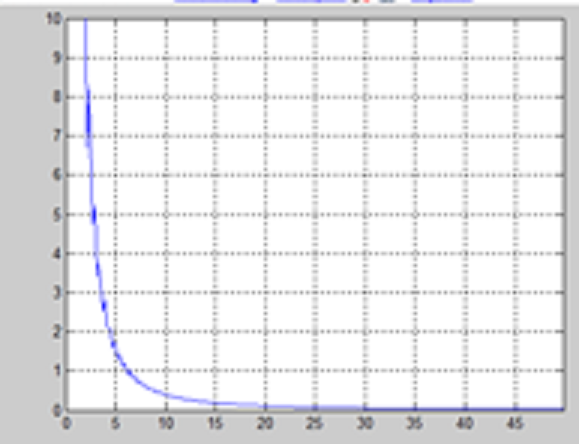
\includegraphics[angle=0, scale = 0.9]{13.png}\newline
рис. 13   спектр треугольного сигнала\newline
\end{center}
\end{figure}

\begin{figure}
\begin{center}
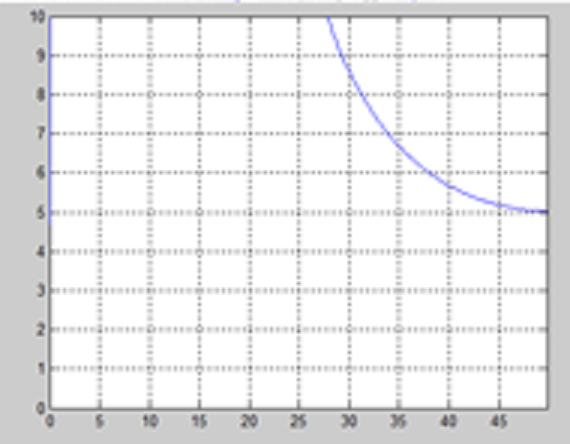
\includegraphics[angle=0, scale = 0.9]{14.png}\newline
рис. 14   спектр прямоугольного сигнала\newline
\end{center}
\end{figure}

\begin{figure}
\begin{center}
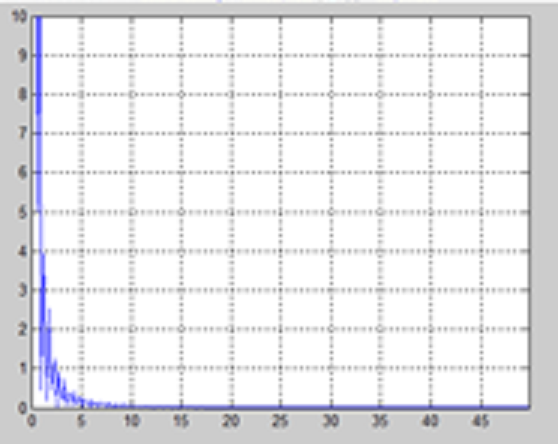
\includegraphics[angle=0, scale = 0.79]{15.png}\newline
рис. 15    спектр полигармонического сигнала\newline
\end{center}
\end{figure}

\begin{figure}
\begin{center}
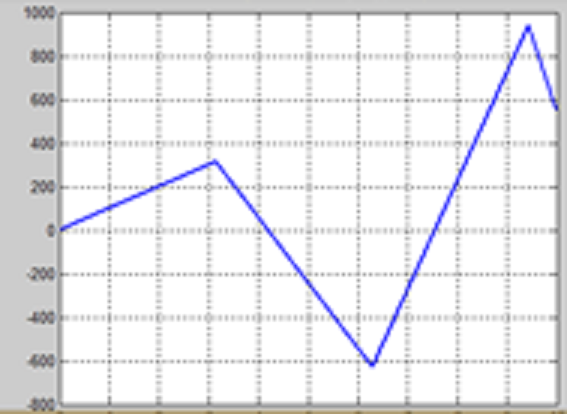
\includegraphics[angle=0, scale = 0.9]{16.png}\newline
рис. 16    треугольный сигнал\newline
\end{center}
\end{figure}
\chapter{Линейная фильтрация}
\section{Алгоритм работы}
Сгенерировать гармонический сигнал с шумом и синтезировать ФНЧ. Получить сигнал во временной и частотной областях до и после фильтрации. Сделать выводы о воздействии ФНЧ на  спектр сигнала.
\section{Код MATLAB}
function seti6() \newline

x = 0:0.01:4*pi;\newline
f=100*(0:255)/512;\newline
figure(1)\newline
noise=rand(size(x));\newline
y = sin(2*pi*x);\newline
ynoisy = y+0.3*noise;\newline
plot(x(1:200),y(1:200))\newline
title('Исходный сигнал')\newline
grid\newline
figure(2)\newline
plot(x(1:200),ynoisy(1:200))\newline
title('Исходный сигнла с шумом')\newline
grid\newline
[B,A] = butter(16,0.98); % Синтез ФНЧ Баттерворта\newline
B=B./sum(B);\newline
A=A./sum(A);\newline
%Обработка сигнала ФНЧ\newline
figure(3)\newline
yfiltered = conv(ynoisy,[B,A]);\newline
plot(x(1:200),yfiltered(1:200))\newline
title('Отфильтрованный зашумленный сигнал')\newline
grid\newline
figure(4)\newline
normalspectrum = fft(y,512);\newline
normspectrum = normalspectrum.*conj(normalspectrum)/512;\newline
plot(f,normspectrum(1:256))\newline
axis([0 max(f) 0 2])\newline
title('Спектр исходного сигнала')\newline
grid\newline
figure(5)\newline
noisyspectrum = fft(ynoisy,512);\newline
normnoisyspectrum = noisyspectrum.*conj(noisyspectrum)/512;\newline
plot(f,normnoisyspectrum(1:256))\newline
axis([0 max(f) 0 2])\newline
title('Спектр зашумленного сигнала')\newline
grid\newline
figure(6)\newline
spectrum = fft(yfiltered,512);\newline
normfilteredspectrum=spectrum.*conj(spectrum)/512;\newline
plot(f,normfilteredspectrum(1:256))\newline
axis([0 max(f) 0 2])\newline
title('Спектр отфильтрованного сигнала')\newline
grid\newline
end\newline
\section{Результаты работы}
\begin{figure}
\begin{center}
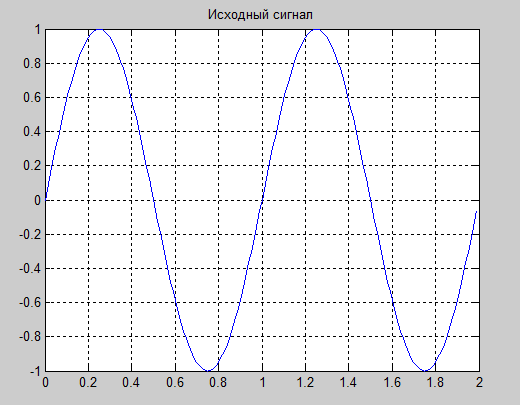
\includegraphics[angle=0, scale = 0.9]{6_1.png}\newline
рис.17. Исходный сигнал\newline
\end{center}
\end{figure}
\begin{figure}
\begin{center}
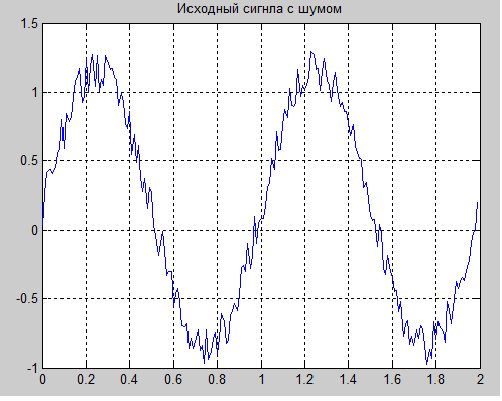
\includegraphics[angle=0, scale = 0.9]{6_2.png}\newline
рис.18. Зашумленный сигнал\newline
\end{center}
\end{figure}
\begin{figure}
\begin{center}
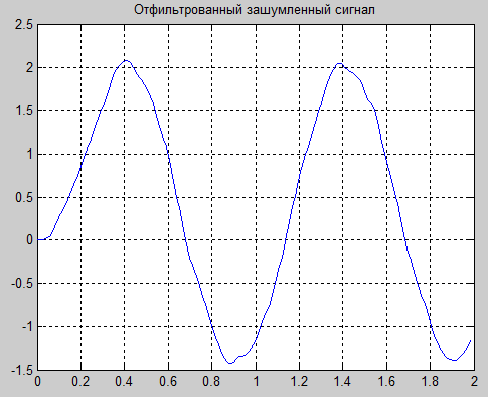
\includegraphics[angle=0, scale = 0.9]{6_3.png}\newline
рис.19. Отфильтрованный сигнал\newline
\end{center}
\end{figure}
\begin{figure}
\begin{center}
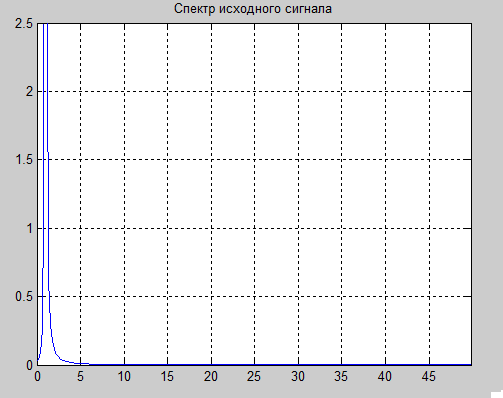
\includegraphics[angle=0, scale = 0.9]{6_4.png}\newline
рис.20. Спектр исходного сигнала\newline
\end{center}
\end{figure}
\begin{figure}
\begin{center}
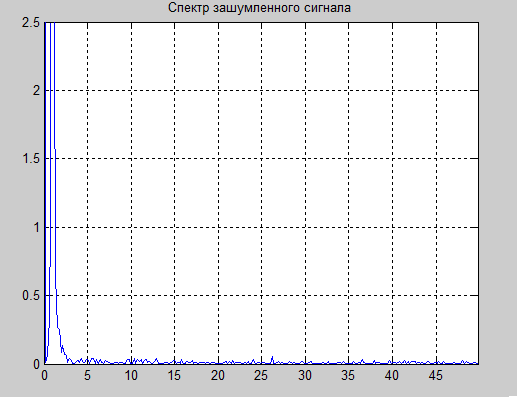
\includegraphics[angle=0, scale = 0.9]{6_5.png}\newline
рис.21. Спектр зашумленного сигнала\newline
\end{center}
\end{figure}
\begin{figure}
\begin{center}
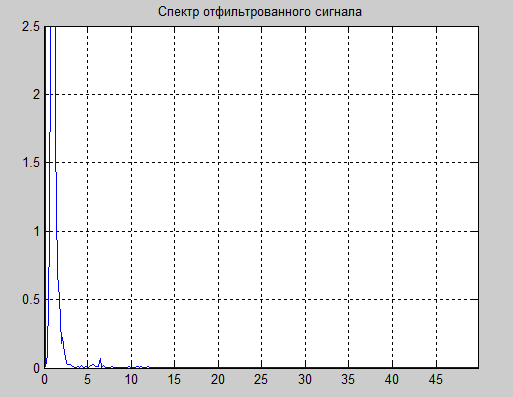
\includegraphics[angle=0, scale = 0.9]{6_6.png}\newline
рис.21. Спектр отфильтрованного сигнала\newline
\end{center}
\end{figure}

\chapter{Аналоговая модуляция}
\section{Алгоритм работы}
\begin{itemize}
	\item Сгенерировать однотональный сигнал низкой частоты.
	\item Выполнить амплитудную модуляцию, используя встроенную функцию MATLAB.
	\item Получить спектр модулированного сигнала. 
	\item Выполнить модуляцию с подавлением несущей. 
	\item Получить спектр. 
	\item Выполнить однополосную модуляцию
	\item Выполнить синхронное детектирование и получить исходный однополосный сигнал
	\item Расчитать КПД модуляции
\end {itemize}
\section{Код MATLAB}
function seti7() \newline
close all;\newline
x = 0:0.01:4*pi;\newline
f0 = 0.5;\newline

y = sin(2*pi*f0*x);\newline
figure(1)\newline
plot(x(1:1000),y(1:1000), 'LineWidth', 1)\newline
title('Однотональный сигнал низкой частоты')\newline
grid\newline

spectrum = fft(y, 1024);\newline
normspectrum = spectrum.*conj(spectrum)/1024;\newline
f = 100*(0:255)/1024;\newline
figure(2)\newline
plot(f, normspectrum(1:256), 'LineWidth', 1)\newline
axis([0 max(f) 0 150])\newline
title('Спектр исходного сигнала')\newline
grid\newline

Fc = 10*f0;\newline
Fs = 100*f0;\newline
U = ammod(y, Fc, Fs, 0, 1);\newline
figure(3)\newline
plot(x(1:1000), U(1:1000),  'LineWidth', 1)\newline
title('Модулированный сигнал')\newline
grid\newline

uspectrum = fft(U, 1024);\newline
normuspectrum = uspectrum.*conj(uspectrum)/1024;\newline
figure(4)\newline
plot(f, normuspectrum(1:256))\newline
axis([0 max(f) 0 70])\newline
title('Спектр модулированного сигнала')\newline
grid\newline

Fc = 10*f0;\newline
Fs = 100*f0;\newline
U = ammod(y, Fc, Fs);\newline
figure(5)\newline
plot(x(1:1000), U(1:1000), 'LineWidth', 1)\newline
title('Модуляция с подавлением несущей')\newline
grid\newline

uspectrum = fft(U, 1024);\newline
normuspectrum = uspectrum.*conj(uspectrum)/1024;\newline
figure(6)\newline
plot(f, normuspectrum(1:256))\newline
axis([0 max(f) 0 70])\newline
title('Спектр модулированного сигнала с подвалением несущей')\newline
grid\newline
\newline
Fc = 10*f0;\newline
Fs = 100*f0;\newline
U = ssbmod(y, Fc, Fs, [], 'upper');\newline
figure(7)\newline
plot(x(1:500), U(1:500), 'LineWidth', 1)\newline
title('Однополосая модуляция')\newline
grid\newline

uspectrum = fft(U, 1024);\newline
normuspectrum = uspectrum.*conj(uspectrum)/1024;\newline
figure(8)\newline
plot(f, normuspectrum(1:256))\newline
axis([0 max(f) 0 70])\newline
title('Спектр однополосной модуляции')\newline
grid\newline

[b, a] = butter(10, Fc*2/Fs);\newline
z = ssbdemod(U, Fc, Fs, 0, b, a);\newline
figure(9)\newline
plot(x(1:1000), z(1:1000), 'LineWidth', 1)\newline
title('Синхронное детектирование')\newline
grid\newline

duspectrum = fft(U, 1024);\newline
normduspectrum = duspectrum.*conj(duspectrum)/1024;\newline
figure(10)\newline
plot(f, normduspectrum(1:256))\newline
axis([0 max(f) 0 70])\newline
title('Спектр детектированного сигнала')\newline
grid\newline

M = 0.5;\newline
n = M*M/(M*M+2)\newline
end

\section{Результаты работы}
\begin{figure}
\begin{center}
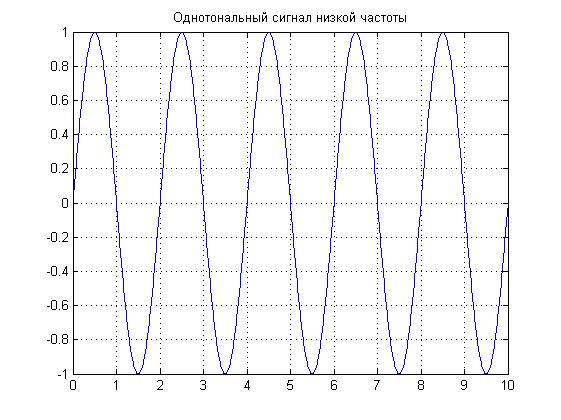
\includegraphics[angle=0, scale = 0.9]{7_1.jpg}\newline
рис. Исходный сигнал\newline
\end{center}
\end{figure}
\begin{figure}
\begin{center}
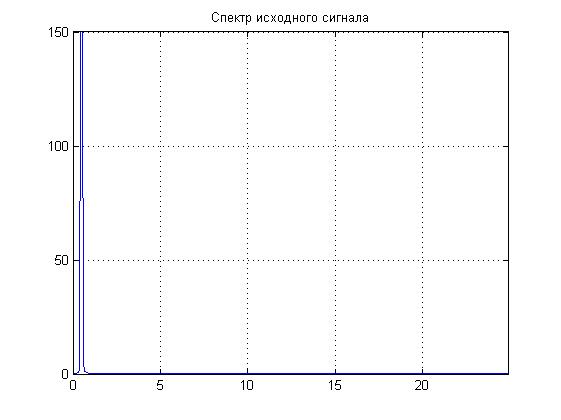
\includegraphics[angle=0, scale = 0.9]{7_2.jpg}\newline
рис. спектр исходного сигнала\newline
\end{center}
\end{figure}
\begin{figure}
\begin{center}
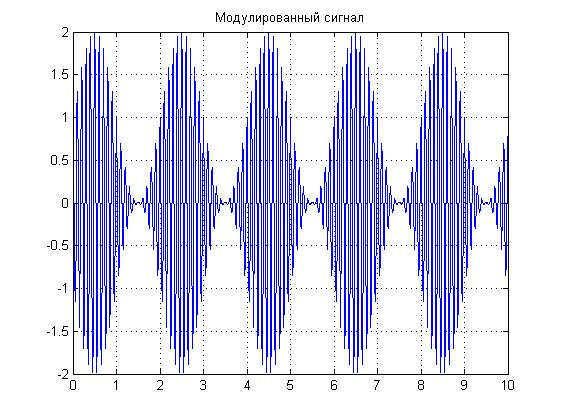
\includegraphics[angle=0, scale = 0.9]{7_3.jpg}\newline
рис. Модулированный сигнал\newline
\end{center}
\end{figure}
\begin{figure}
\begin{center}
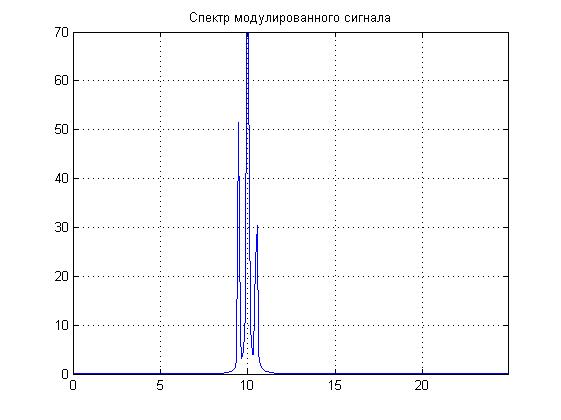
\includegraphics[angle=0, scale = 0.9]{7_4.jpg}\newline
рис. Спектр модулированного сигнала\newline
\end{center}
\end{figure}
\begin{figure}
\begin{center}
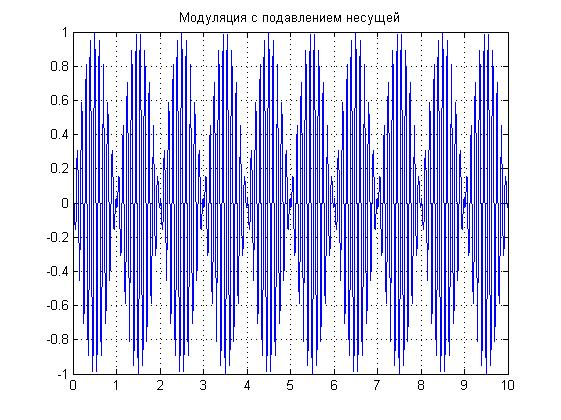
\includegraphics[angle=0, scale = 0.9]{7_5.jpg}\newline
рис. Сигнал с подавлением несущей\newline
\end{center}
\end{figure}
\begin{figure}
\begin{center}
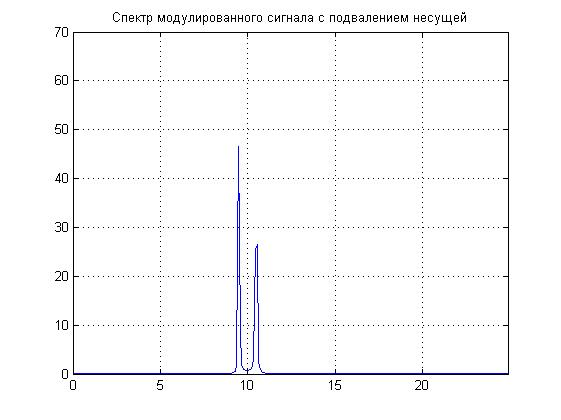
\includegraphics[angle=0, scale = 0.9]{7_6.jpg}\newline
рис. Спектр сигнала с подавлением несущей\newline
\end{center}
\end{figure}
\begin{figure}
\begin{center}
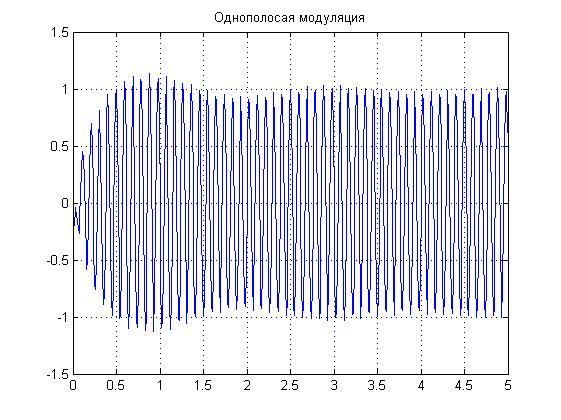
\includegraphics[angle=0, scale = 0.9]{7_7.jpg}\newline
рис. Одгополосный сигнал\newline
\end{center}
\end{figure}
\begin{figure}
\begin{center}
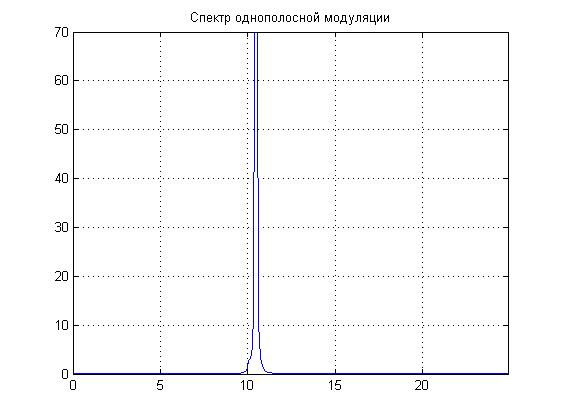
\includegraphics[angle=0, scale = 0.9]{7_8.jpg}\newline
рис. Спектр однополосного сигнала\newline
\end{center}
\end{figure}
\begin{figure}
\begin{center}
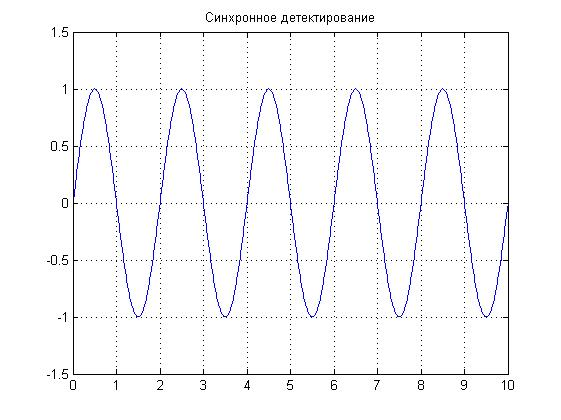
\includegraphics[angle=0, scale = 0.9]{7_9.jpg}\newline
рис.детектированный сигнал\newline
\end{center}
\end{figure}
\begin{figure}
\begin{center}
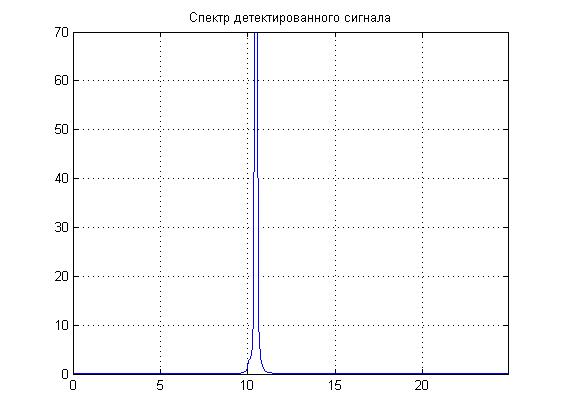
\includegraphics[angle=0, scale = 0.9]{7_10.jpg}\newline
рис. Спектр детектированного сигнала\newline
\end{center}
\end{figure}
\begin{figure}
\begin{center}
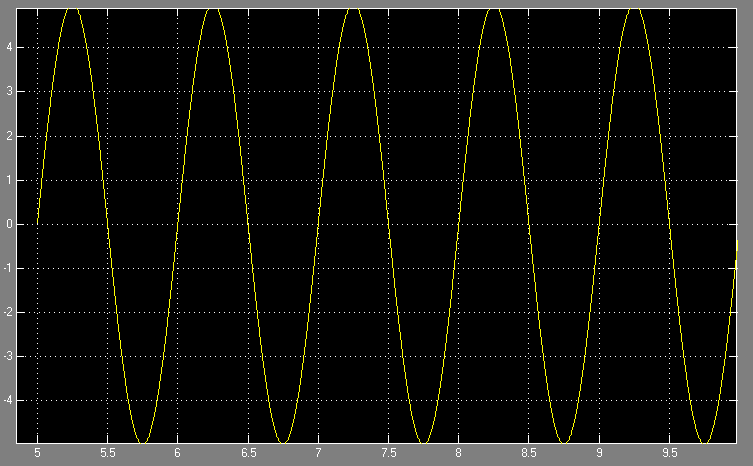
\includegraphics[angle=0, scale = 0.9]{7_11.png}\newline
рис. Исходный сигнал. Simulink\newline
\end{center}
\end{figure}
\begin{figure}
\begin{center}
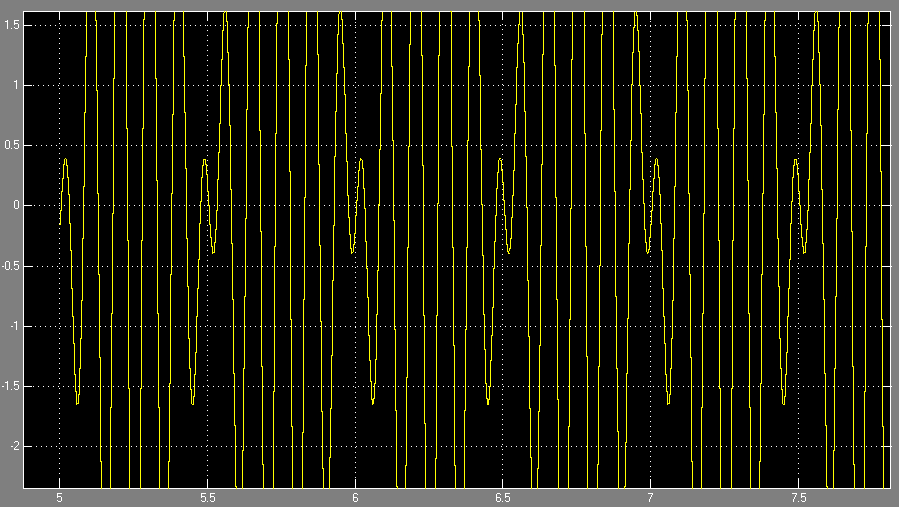
\includegraphics[angle=0, scale = 0.9]{7_12.png}\newline
рис.Модуляция Simulink\newline
\end{center}
\end{figure}
\begin{figure}
\begin{center}
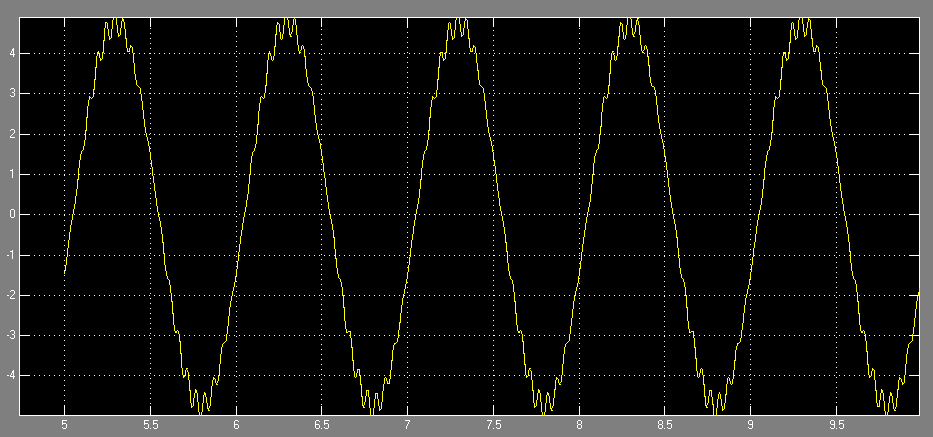
\includegraphics[angle=0, scale = 0.9]{7_13.png}\newline
рис.Демодуляция. Simulink\newline
\end{center}
\end{figure}
\begin{figure}
\begin{center}
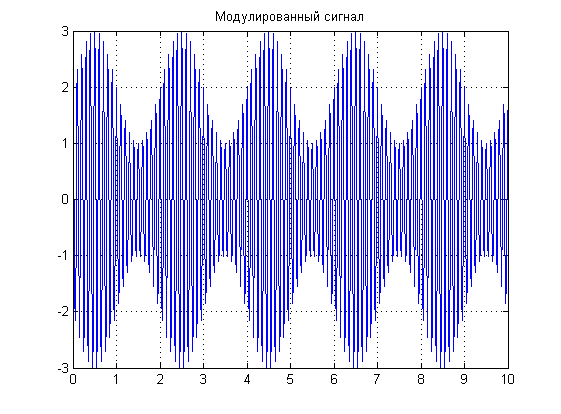
\includegraphics[angle=0, scale = 0.9]{7_14.png}\newline
рис. Модулированный сигнал с коэффициентом 2\newline
\end{center}
\end{figure}
\begin{figure}
\begin{center}
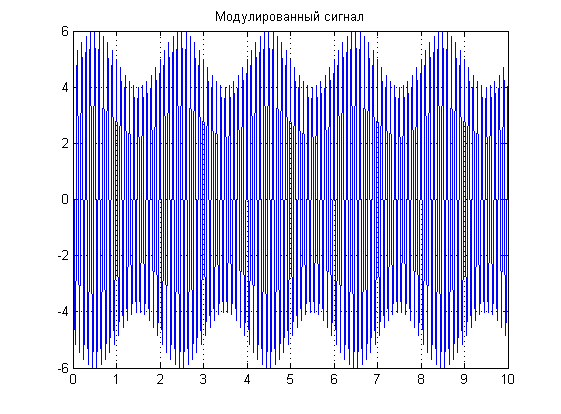
\includegraphics[angle=0, scale = 0.9]{7_15.png}\newline
рис. Модулированный сигнал с коэффициентом 5\newline
\end{center}
\end{figure}
\chapter{Вывод}
В данной лабораторной работе был получен спектр исходного сигнала и спектр зашумленного сигнала. Полученный спектр представляет собой одну гармонику синуса с определенной частотой, что объясняется наличием у сигнала одной частоты. Теоретически ожидалось получить один спектр, практически был получен спектр, который представляет собой узкую полоску на графике. Практические результаты оказались очень правдивыми. После нанесения шума на сигнал, был получен спектр зашумленного сигнала. Спектр зашумленного сигнала представляет собой прерывистые линии на графике. Таким образом спектр сигнала также оказался зашумленным. \newline

В следующей лабораторной работе было проведено моделирование полигармонического сигнала

 прямоугольного сигнала и треугольного сигнала. Были получены спектры данных сигналов. Для получения сигналов использовались математические формулы данных функций, а также средство моделирования Simulink. Обоими способами были получены спектры сигналов. Частным случаем в работе было получение треугольного сигнала через премение операции свертки над произведением двух прямоуголных сигналов. Данная операция осуществляется как математически, так и при моделировании в среде Simulink.
Обоснованием получения треугольного сигнала из свертки двух прямоугольных служит тот факт, что интеграл от произведения двух констант есть линейная функция. График такого преобразования будет представлять две линеных функции, одна из котрых имеет положительный коэффициента наклона, а другая отрицательный.

В шестой лабораторной работе были исследованы синтез фильтра Баттерворта 16 порядка и фильтрация зашумленного сигнала с помощью данного фильтра.
При фильтрации сигнала происходит игнорировнаие ненужных частот(частот шума), после чего сигнал преобретает более понятную форму, близкую к исходному. При этом фильтр
полностью не срезает все ненужные частоты в сигнале, это связано с заданной посой пропускания, которая пропускает все частоты, что по своему значению больше заданной полосы пропускания.
Также неполное срезание частот связано с тем, что вследствие нерезкого падения графика срезания частот самого фильтра, он успевает захватить еще несколько частот. 
Вследствие чего, данный фильтр не избавляет сигнал от шумов полностью.

В седьмой лабораторной работе были исследованы различные типы аналоговой модуляции (амплитудная, частотная, фазовая). В процессе модуляции исходного сигнала у него 
изменяются следующие параметры: амплитуда, частота и фаза. В ходе работы был поставлен опыт по изменению коэффициента модуляции с содержанием несущего сигнала.
При увеличении данного параметра модуляция переносит исходный сигнал на более высокие частоты. при этом спектр модулированного сигнала представляет собой 3 вертикальных полосы, 
две из которых симметрично расположены относительно средней. Средняя полоса обозначает спектр несущего сигнала. В ходе работы была произведена модуляция с подавлением несущей.
При этом происходит игнорирование несущего сигнала, который является основным источником информации по передаваемому каналу. Спектр такого сигнала представляет собой 2 вертикальных
 симметричных полосы, что говорит об отсутствии несущего сигнала. В работе была проведена модуляция однополосного сигнала. Данный сигнал используется для уменьшения мошности 
потребления энергии для переноса информации и для осуществления переноса информации на более дальние расстояния. Спектр такого сигнала представляет собой одну полосу,
так как в нем исключены несущий сигнал и половина исходного. Также было произведено детектирование сигнала, в результате которого из модулированного сигнала был получен исходный сигнал
со своим спектром и свойствами. Спектр полученного сигнала отличается от начального. В результате вычисления КПД установлено, что с ростом коэффициента модуляции 
растет и КПД сигнала, что сказывается на более точной передачи информации.
КПД = 0.9259 для коэффициента = 5.
\begin{figure}
\begin{center}
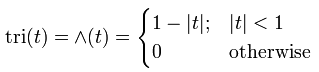
\includegraphics[angle=0, scale = 0.8]{17.png}\newline
рис. 17    Формула полигармонического сигнала\newline
\end{center}
\end{figure}
\begin{figure}
\begin{center}
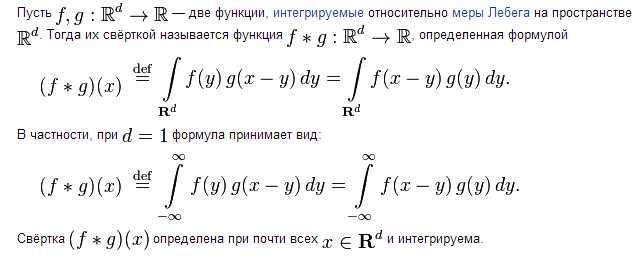
\includegraphics[angle=0, scale = 0.8]{18.png}\newline
рис.   Свертка функций
\end{center}
\end{figure}
\begin{figure}
\begin{center}
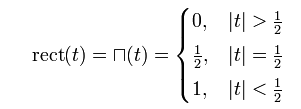
\includegraphics[angle=0, scale = 0.8]{19.png}\newline
рис.    Прямоугольная функция
\end{center}
\end{figure}
\begin{figure}
\begin{center}
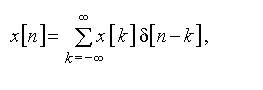
\includegraphics[angle=0, scale = 0.8]{20.png}\newline
рис.    Спектр сигнала. Математическое представление \newline
\end{center}
\end{figure}

\end{document}


